\documentclass[11pt, a4paper, oneside]{report}

\usepackage[francais]{babel}
\usepackage[T1]{fontenc}
\usepackage[utf8]{inputenc}

\usepackage[left=2cm, right=2cm, top=2cm, bottom=2cm]{geometry}
\usepackage{fancyhdr}
\usepackage{lastpage}
\usepackage{hyperref}

\usepackage{graphicx}
\usepackage{tikz}
\usepackage{pgfgantt}

\usepackage{perpage} %the perpage package
\MakePerPage{footnote} %the perpage package command

\usepackage{color}
\usepackage{colortbl}

\usepackage{float}

\usepackage{makeidx}

\usepackage{listings}
\usepackage{CJKutf8}

\usepackage{tabularx}
\usepackage{multicol}

\usepackage{pgfgantt} % planning gantt

%arborescence
\usepackage{dirtree}

\usepackage{subfigure}

\usepackage{enumitem}
\setlist[description]{leftmargin=\parindent,labelindent=\parindent}

\usepackage{etoolbox}
\patchcmd{\chapter}{\thispagestyle{plain}}{\thispagestyle{fancy}}{}{}

\usepackage{ragged2e}  % for '\RaggedRight' macro (allows hyphenation)
\newcolumntype{Y}{>{\RaggedRight\arraybackslash}X} 

\newcommand{\HRule}{\rule{\linewidth}{0.5mm}}

\makeindex
\makeatletter
\renewenvironment{theindex}
{
    \thispagestyle{fancy}
    \setlength{\parindent}{0pt}
    \let
    \item
    \@idxitem
}{\onecolumn}
\makeatother

\setlength{\parindent}{0cm}

\lstset{
    basicstyle=\ttfamily,
    stringstyle=\ttfamily\color{green!50!black},
    keywordstyle=\bfseries\color{blue},
    commentstyle=\itshape\color{red!50!black},
    showstringspaces=true,
    tabsize=4,
    frame=single,
    numbers=left,
    numberstyle=\tiny,
    firstnumber=1,
    stepnumber=1,
    numbersep=5pt,
    breaklines=true
}

\graphicspath{{img/}}

\pagestyle{fancy}
\setlength{\headheight}{14pt}
\renewcommand{\headrulewidth}{0.5pt}
\lhead{Yannick Brodard}
\chead{\leftmark}
\rhead{\today}
\renewcommand{\footrulewidth}{0.5pt}
\lfoot{CFPT - École d'informatique}
\cfoot{Travail de diplôme}
\rfoot{Page \thepage ~sur \pageref{LastPage}}

\newcommand{\teacherlastname}{Maréchal}
\newcommand{\teacherfirstname}{Christophe}
\newcommand{\teacheremail}{christophe.marechal@edu.ge.ch}

\newcommand{\school}{CFPT-EI}
\newcommand{\schoolyear}{2014-2015}

\newcommand{\candidatelastname}{Brodard}
\newcommand{\candidatefirstname}{Yannick}
\newcommand{\candidatephone}{+41 79 137 67 11}
\newcommand{\candidateemail}{yannick.r.brodard@gmail.com}

\newcommand{\projectTitle}{Hel}
\newcommand{\projectSubTitle}{The pixelated horror}

% Niveau table des matières
\setcounter{tocdepth}{3}
% --------------------------------------------------
\begin{document}
% --------------------------------------------------
\begin{titlepage}
	\begin{center}
		\vspace*{\fill}
		
\includegraphics[width=.5\textwidth]{cfpt_logo}\\[.4cm]
		\textsc{\Large Centre de formation professionnelle technique\\École d'informatique}\\[.4cm]
		\textsc{\Large Travail de diplôme}\\[.1cm]
		\textsc{\Large Documentation}\\[0.4cm]
		\textsc{\large \schoolyear}\\[0.4cm]
		
		% Title
		\HRule \\[0.4cm]
		{ \huge \bfseries \projectTitle \\[0.4cm] }
		{ \Large \bfseries \emph{\projectSubTitle} \\[0.4cm] }
		\HRule \\[1.5cm]
		
		% Author and supervisor
		\noindent
		\begin{minipage}{0.4\textwidth}
		\begin{flushleft} \large
		\emph{Auteur:}\\
		\candidatefirstname \textsc{~\candidatelastname}\\[0.2cm]
		{\small
		\texttt{\candidateemail}\\
		\texttt{\candidatephone}
		}
		\end{flushleft}
		\end{minipage}%
		\begin{minipage}{0.4\textwidth}
		\begin{flushright} \large
		\emph{Superviseur:} \\
		\teacherfirstname \textsc{~\teacherlastname}\\[0.2cm]
		{\small
		\texttt{\teacheremail}\\
		~
		}
		\end{flushright}
		\end{minipage}
		
		\vspace*{\fill}
		
		% Bottom of the page
		{\large \today}
		
	\end{center}
\end{titlepage}
% --------------------------------------------------
\chapter{Avant-propos}
\section{Résumé}
\section{Abstract}
\newpage
% --------------------------------------------------
\tableofcontents
\newpage
% --------------------------------------------------
\chapter{Cahier des charges}
\section{But}
L'objectif est de créer un jeu divertissant pour le joueur moyen. \projectTitle\footnote{\textit{\projectTitle} : Nom du jeu-vidéo et aussi nom de la déesse de la mort dans la mythologie nordique} doit être bien construit et doit avoir la possibilité d'ajouter du contenu facilement.\\[.5cm]
Le jeu-vidéo est en deux dimensions (2D) avec une vue de dessus\footnote{Une vue de dessus peut être comparable au jeu Dwarf Fortress. Voir voir Figure \ref{fig:df} page \pageref{fig:df}} et inclue quelques aspects d'un jeu RPG\footnote{Rôle Playing Game : Un RPG est un jeu où le joueur fait évoluer son personnage avec ses choix et/ou ses compétences.}. L'utilisateur contrôle un personnage qui se retrouve coincé dans une pièce inconnue et doit s'aventurer dans cet environnement inconnu et découvrir ses mystères. Cette salle contient des ennemis que le joueur peut contourner ou vaincre. Grâce à ceci, le héros gagne des points de compétences qu'il peut dépenser pour augmenter ses capacités une fois que le joueur meurt. Quand le joueur meurt, celui-ci réapparaît au début de cette salle, mais sans perdre ses compétences, d'une part la pièce aura aussi changé. Des éléments de celui-ci auront disparu ou bougé et d'autres auront apparu. L'utilisateur devra s'aventurer dans cet endroit mystérieux pour essayer de trouver une sortie. Une fois que le joueur a trouvé la sortie, il affrontera \emph{Hel}, la déesse de la mort seulement après l'avoir vaincu qu'il pourra sortir de cette salle, mais si le héros meurt pendant l'affrontement, il devra recommencer depuis le début et perdra tous ses points de compétences.

\begin{figure}[h]
	\begin{center}
	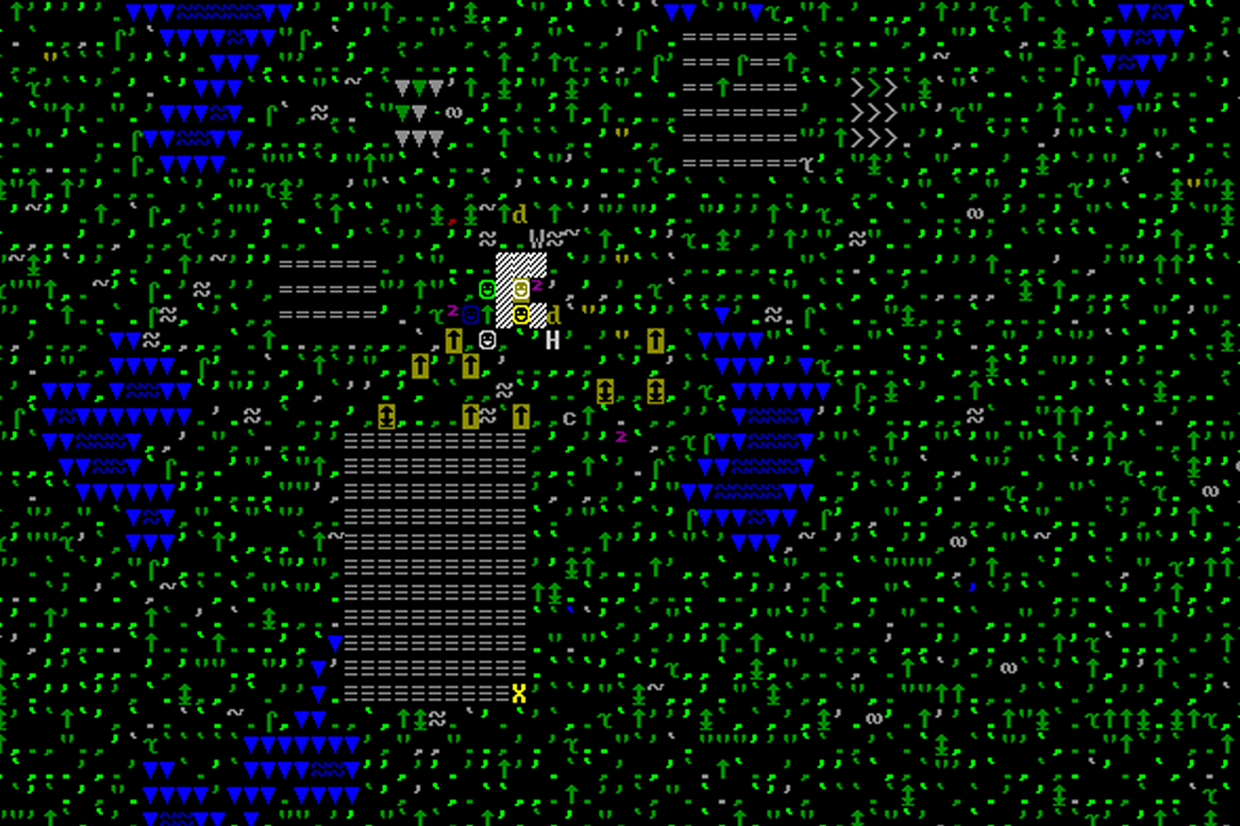
\includegraphics[width=0.45\textwidth]{df}
	\caption{Dwarf Fortress - Jeu en pixel art fait par \textit{Bay 12 Games}}
	\label{fig:df}
	\end{center}
\end{figure}

\projectTitle~est principalement inspiré du jeu \emph{Don't Move} par "stvr" (voir Figure \ref{fig:dontmove} page \pageref{fig:dontmove}). \emph{Don't Move} est un jeu indépendant qui a reçu de très bonnes critiques. Le concept du jeu est simple, si le joueur bouge, il meurt, mais en faisant cela il débloque de nouvelles fonctionnalités du jeu et de nouveaux objectifs. Le but de \projectTitle~est de pousser ce concept encore plus loin et de l'améliorer avec plus de fonctionnalités.

\begin{figure}[h]
	\begin{center}
	
\includegraphics[width=0.265\textwidth]{dontmove}
	\caption{Don't Move - jeu indépendant développé par "stvr"}
	\label{fig:dontmove}
	\end{center}
\end{figure}

\section{Description détaillée}
\projectTitle~est un jeu solo (1 joueur seulement) qui est en deux dimensions. Le jeu sera développé de manière dynamique et générique qui permettra de facilité l'ajout de contenu. Ce contenu peut être :
\begin{multicols}{2}
\begin{itemize}
	\item des armes
	\item des ennemis
	\item des nouvelles compétences
	\item de nouveaux types de points de compétences
	\item des objets de la salle
	\item des différentes disposition de la salle
	\item de nouvelles règles de jeu
\end{itemize}
\end{multicols}

\subsection{Règles}
\begin{description}
	\item Le joueur peut : sauter, se déplacer sur l'axe X, se baisser (ceci active la furtivité), attaquer avec une arme, attaquer avec de la magie et bloquer des attaques pour minimiser les dégâts.
	\item Le joueur a 100 points de vie par défaut.
	\item Les dégâts et vie des ennemis seront à définir selon le meilleur équilibre de jeu.
	\item Le joueur possède des sorts qu'il peut placer dans les touches attribuées pour les enclencher.
\end{description}

\subsection{Méchanismes}
\subsubsection{Salle}
La salle du jeu change à chaque fois que le joueur meurt. Cette salle peut avoir de nouveaux éléments, de nouvelles textures ou même de nouveaux ennemis.

\subsubsection{Points de compétences}
Le joueur peut gagner des points de compétences en tuant des ennemis ou en trouvant des pièces qui se trouve un peu partout dans la salle. Ces pièces sont défendu par des ennemis et peuvent disparaître si le joueur n'est pas discret. Il ne peut dépenser ces points après sa mort. 

\subsubsection{Compétences}
Avant de réapparaître en jeu, le joueur peut attribuer ces points sur des compétences du personnage. Par exemple, le joueur peut dépenser 2 points de compétences sur la compétence "Force" pour avoir plus de dégâts sur les coups du personnage. Voici une liste des compétences :

\begin{center}
\begin{tabularx}{\textwidth}{l X}
	\hline
	\textbf{Compétence} & \textbf{Description}\\
	\hline \hline
	Force & Apporte plus de dégâts sur les coups physiques du personnage.\\
	Agilité & Les ennemis remarquent moins le joueur et celui-ci peut se déplacer plus rapidement\\
	Vitalité & Apporte plus de points de vie au joueur\\
	Magie & Apporte plus de dégâts pour les attaques magiques du joueur\\
	\hline
\end{tabularx}
\end{center}

\subsubsection{Armes}
Les armes sont des objets pouvant être récoltés en explorant la salle. Quand le joueur trouve une arme, cette arme est mise dans l'inventaire du joueur. Le joueur pourra équiper l'arme pour faire plus de dégâts. Les armes ont des statistiques qui augmentent les dégâts physiques et/ou magiques.

\subsubsection{Sorts}
Les sorts sont des pouvoirs magiques que le joueur peut utiliser contre ses ennemis. Les dégâts magiques sont augmentés selon les points de compétences attribués à la magie. Des sorts peuvent être trouvés dans la salle sous forme de parchemin que le joueur peut ramasser, les sorts se placent dans l'inventaire et peuvent être attribués à des touches d'action (Maximum 4, touches par défaut : 1, 2, 3 ,4).

\subsection{Contrôles}
\begin{table}[htp]
\begin{center}
\begin{tabular}{|c|l|}
	\hline
	\textbf{Touche} & \textbf{Description}\\
	\hline \hline
	W & Sauter\\
	\hline
	A & Aller à gauche\\
	\hline
	D & Aller à droite\\
	\hline
	S & Se baisser (mode furtif)\\
	\hline
	Clique gauche & Attaquer (dégâts physique)\\
	\hline
	1 & Sort numéro 1\\
	\hline
	2 & Sort numéro 2\\
	\hline
	3 & Sort numéro 3\\
	\hline
	4 & Sort numéro 4\\
	\hline
	I & Afficher l'inventaire\\
	\hline
	ESC & Afficher le menu (met le jeu en pause)\\
	\hline
\end{tabular}
\end{center}
\caption{Contrôles de bases du jeu}
\end{table}
\subsection{Interface utilisateur}
L'interface utilisateur doit permettre au joueur de régler plusieurs paramètres et exécuter des actions.

\subsubsection{Options}
Les options de son, vidéo, difficulté et attribution des touches de jeu doivent être disponibles.
\subsubsection{Actions}
Il doit être possible de commencer, sauvegarder et charger une partie, puis de visualiser les scores obtenus des parties terminées.

\section{Environnement de travail}
\subsection{Inventaire hardware}
\begin{itemize}
	\item Intel Core i7 2600K @ 3.40GHz
	\item 8.00Go Dual-Channel DDR3 @ 823MHz
	\item 1024MB NVIDIA GeForce GTX 550 Ti
\end{itemize}

\subsection{Inventaire software}
\begin{itemize}
	\item Visual Studio 2013 Professional
	\item MonoGame (C\#)
\end{itemize}

\subsection{Durée et dates du projet}
Le projet se déroule sur une période de 7 semaines avec 40 heures de travail par semaine. Il y a aussi 3 jours fériés pendant le projet. Ce qui fait un total de 256 heures de travail.\\[0.3cm]
Le projet commence le lundi, 13 avril 2015 avec une reddition intermédiaire (documentation + poster) le jeudi, 30 avril 2015, puis la reddition finale le lundi, 1\textsuperscript{er} juin 2015.
\newpage
% --------------------------------------------------
\chapter{Analyse préliminaire}
\section{Analyse de l'existant}
Il n'est pas anodin de trouver des jeux similaires dans le marché du jeu-vidéo, en effet, beaucoup d'indépendants et des grandes entreprises produisent ces divertissements. Parmi les plus connus qui peuvent ressembler à \projectTitle, il existe \emph{Diablo III} et \emph{Path of Exile} qui sont des jeux récents. Ils sont similaires par rapport au type de jeu, ce sont des RPG et des Hack and Slash.

\emph{Bastion} et \emph{Transistor} sont également des jeux RPG et indépendant créer par la petite entreprise \emph{Supergiant Games}. Ces jeux sont prisés pour leur art, richesse graphique et histoire passionnante.
\section{Critique de l'existant}
\textbf{Diablo III} par \emph{Blizzard Entertainment} est actuellement le poids-lourd dans ce type de jeu, avec de hautes qualités graphiques, un contenu riche et une grande communauté active. Il est critiqué de ne pas être assez complexe et d'être trop facile à battre. 

\textbf{Path of Exile} par \emph{Grinding Gear Games} est le concurrent direct de \emph{Diablo III}, il est valorisé avec sa complexité technique dans le gameplay. Il est critiqué de ne pas être assez accessible aux joueurs lambdas et d'être trop difficile.

\textbf{Bastion} par \emph{Supergiant Games} est un jeu indépendant ayant gagné plusieurs titres pour sont originalité.
\section{Différentiation du projet}

\newpage
% --------------------------------------------------
\chapter{Analyse fonctionnelle}
\section{Personnage}
\subsection{Général}
Un personnage est contrôlé par le joueur, celui-ci peut l'équiper avec divers objets trouvé dans la salle pour augmenter ses caractéristiques. Il peut utiliser des sorts et ses armes pour vaincre ses ennemis. Le personnage possède \textbf{100} points de vie par défaut, ces points de vie augmente si le joueur décide d'améliorer sa vitalité avec des points de compétences ou des objets.

Le personnage possède 4 compétences de bases (voir section \ref{sec:competences}), il peut gagner des compétences en tuant des ennemis ou en trouvant des pièces dans la salle.

Il possède \textbf{200} points de mana qu'il peut dépenser pour utiliser des sorts. Le mana se régénéré avec le temps de \textbf{20} points de mana par seconde. 
\subsection{Inventaire}
Le personnage possède un inventaire qui sert à stocker ses objets sur soi. Les objets stocké dans l'inventaire prennent une certaine place à l'intérieur. Il n'est pas de taille infini.
\section{Compétences}
\label{sec:competences}
Les compétences sont des caractéristiques pouvant être augmenter par le personnage. Ils permettent d'augmenter ses capacités. Il existe plusieurs compétences qui sont :

\begin{description}
	\item[Force] Apporte plus de dégats sur les coups physiques
	\item[Agilité] Le personnage est plus discret et peut se déplacer plus rapidement
	\item[Vitalité] Augmente les points de vie du personnage
	\item[Magie] Augmente les dégâts magiques du personnage
\end{description}

\begin{figure}[ht]
\centering
\subfigure[Force]{%

\includegraphics[width=.20\textwidth]{strenght}
\label{fig:strenghtlogo}}
\subfigure[Agilité]{%

\includegraphics[width=.20\textwidth]{agility}
\label{fig:agilitylogo}}
\subfigure[Vitalité]{%

\includegraphics[width=.20\textwidth]{vitality}
\label{fig:vitalitylogo}}
\subfigure[Magie]{%

\includegraphics[width=.20\textwidth]{magic}
\label{fig:magiclogo}}
%
\caption{Logos des compétences}
\label{fig:competences}
\end{figure}

\section{Looting}
Le \emph{looting} est le moyen de trouver des objets. Lorsque qu'un ennemi meurt ou que l'on ouvre un coffre, par exemple, celui-ci fait tomber des objet. Cette action est appelée le \emph{looting}.
\section{Caractéristiques}
Les caractéristiques sont des propriétés qui augmente les capacités du personnages. Les compétences sont des caractéristiques mais qui peuvent être augmenter par le héro, alors que les caractéristiques peuvent seulement être augmenter par des objets.\\

\textbf{Liste des caractéristiques}
\begin{description}[labelindent=0.3cm]
    \item[Force] Le nombre de points de compétences de type \emph{Force} ajouté
    \item[Agilité] Le nombre de points de compétences de type \emph{Agilité} ajouté
    \item[Vitalité] Le nombre de points de compétences de type \emph{Vitalité} ajouté
    \item[Magie] Le nombre de points de compétences de type \emph{Magie} ajouté
    \item[Vitesse d'attaque] Le pourcentage de vitesse d'attaque ajouté au personnage
    \item[Vitesse d'attaque initial] La vitesse d'attaque initial du personnage
    \item[Dégâts] Les dégâts infligés après chaque attaque
    \item[Dégâts magiques] Les dégâts magiques infligés après chaque attaque
    \item[Armure] Déduit les dégâts reçu
    \item[Resistance magique] Déduit les dégâts magiques reçu
    \item[Régénération de vie] Régénère les points de vie
    \item[Régénération de mana] Régénère les points de mana
\end{description}
\begin{table}[ht]
\begin{center}
\begin{tabularx}{\textwidth}{| l | Y |}
  \hline                     
  Force 				& Augmente les dégâts de \textbf{1\%}\\ \hline
  Agilité 				& Diminue la distance de vue des ennemi de \textbf{0.0625\%}. Il augmente aussi la vitesse de déplacement de \textbf{0.075\%} \\ \hline
  Vitalité 				& Augmente les points de vie de \textbf{100} \\ \hline
  Magie 				& Augmente les dégâts magiques de \textbf{1\%} \\ \hline
  Vitesse d'attaque 	& Augmente la vitesse d'attaque selon la valeur en \textbf{pourcentage} \\ \hline
  Vitesse d'attaque initial	& Vitesse d'attaque initial du personnage\\ \hline
  Dégâts 				& S'ajoute au dégâts du personnage \underline{avant} d'appliquer la \emph{force} \\ \hline
  Dégâts magiques 		& S'ajoute au dégâts magiques du personnage \underline{avant} d'appliquer la \emph{magie} \\ \hline
  Armure 				& Diminue les dégâts reçu de \textbf{0.075\%} \\ \hline
  Resistance magique 	& Diminue les dégâts magiques reçu de \textbf{0.075\%} \\ \hline
  Régénération de vie 	& Augmente la régénération de points de vie selon la valeur\\ \hline
  Régénération de mana 	& Augmente la régénération de points de mana selon la valeur\\ \hline
\end{tabularx}
\caption{Fonctionnement des caractéristiques}
\end{center}
\end{table}
\section{Équipement}
Les équipements sont des objets que le personnage peut équiper sur lui-même pour augmenter ses points de compétences. Il existe des différents types d'objets.
\begin{itemize}
	\item Accessoires
	\item Armes
	\item Armures
\end{itemize}
%\begin{table}[H]
%\begin{center}
%\begin{tabular}{| l | c | c | c |}
%  \hline      
%  Niveau 				& 1 & 2 & 3\\ \hline \hline                 
%  Force 				& 2 & 3 & 4\\ \hline
%  Agilité 				& 5 & 6 & 4\\ \hline
%  Vitalité 			& 8 & 9 & 4\\ \hline
%  Magie 				& 8 & 9 & 4\\ \hline
%  Vitesse d'attaque 	& 8 & 9 & 4\\ \hline
%  Dégâts 				& 8 & 9 & 4\\ \hline
%  Dégâts magiques 		& 8 & 9 & 4\\ \hline
%  Armure 				& 8 & 9 & 4\\ \hline
%  Resistance magique 	& 8 & 9 & 4\\ \hline
%\end{tabular}
%\caption{Valeurs des caractéristiques}
%\end{center}
%\end{table}
\subsection{Accessoires}
\label{subsec:accessoires}
Les accessoires sont des objets spéciaux qui apporte des capacités spéciales au personnage.
\begin{multicols}{2}
\begin{itemize}
    \item Amulette
    \item Bagues
    \item Carquois
    \item Bouclier
    \item Source de pouvoir
\end{itemize}
\end{multicols}
\subsubsection{Amulette et bagues}
Ces objets apportent aléatoirement 2 à 4 des caractéristiques suivants :
\begin{table}[ht]
\begin{center}
\begin{tabular}{| l | c | c | c |}
  \hline      
  Niveau 				& 1    & 2 & 3\\ \hline \hline                 
  Force 				& 3 - 10 & 15 - 30 & 45 - 100\\ \hline
  Agilité 				& 3 - 10 & 15 - 30 & 45 - 100\\ \hline
  Vitalité 				& 3 - 10 & 15 - 30 & 45 - 100\\ \hline
  Magie 				& 3 - 10 & 15 - 30 & 45 - 100\\ \hline
  Résistance magique 	& 2 - 5  & 10 - 20 & 30 - 55\\ \hline
  Régénération de vie 	& 10 - 80  & 100 - 450 & 500 - 1000\\ \hline
  Régénération de mana 	& 1 - 5  & 6 - 13 & 14 - 20\\ \hline
\end{tabular}
\caption{Valeurs des caractéristiques d'une bague et d'une amulette}
\end{center}
\end{table}
\subsubsection{Carquois}
Le carquois apporte toujours ces caractéristiques :
\begin{multicols}{2}
\begin{itemize}
	\item Vitesse d'attaque
	\item Agilité
\end{itemize}
\end{multicols}
Il apporte aussi 0 à 3 de ces caractéristiques :
\begin{multicols}{2}
\begin{itemize}
    \item Force
    \item Vitalité
    \item Magie
    \item Régénération de vie
    \item Régénération de mana
\end{itemize}
\end{multicols}
\begin{table}[H]
\begin{center}
\begin{tabular}{| l | c | c | c |}
  \hline      
  Niveau 				& 1 & 2 & 3\\ \hline \hline                 
  Force 				& 1 - 5 & 7 - 25 & 35 - 80\\ \hline
  Agilité 				& 3 - 10 & 15 - 30 & 45 - 100\\ \hline
  Vitalité 				& 1 - 5 & 7 - 25 & 35 - 80\\ \hline
  Magie 				& 1 - 5 & 7 - 25 & 35 - 80\\ \hline
  Vitesse d'attaque 	& 1.5\% - 2.0\% & 2.5\% - 3.5\% & 4.0\% - 7.0\%\\ \hline
  Régénération de vie 	& 10 - 80  & 100 - 450 & 500 - 1000\\ \hline
  Régénération de mana 	& 1 - 5  & 6 - 13 & 14 - 20\\ \hline
\end{tabular}
\caption{Valeurs des caractéristiques du carquois}
\end{center}
\end{table}
\subsubsection{Bouclier}
Le bouclier apporte toujours ces caractéristiques :
\begin{multicols}{2}
\begin{itemize}
	\item Armure
	\item Vitalité
\end{itemize}
\end{multicols}
Il apporte aussi 0 à 3 de ces caractéristiques :
\begin{multicols}{2}
\begin{itemize}
    \item Force
    \item Agilité
    \item Magie
    \item Résistance magique
    \item Régénération de vie
    \item Régénération de mana
\end{itemize}
\end{multicols}
\begin{table}[ht]
\begin{center}
\begin{tabular}{| l | c | c | c |}
  \hline      
  Niveau 				& 1 & 2 & 3\\ \hline \hline                 
  Force 				& 1 - 5 & 7 - 25 & 35 - 80\\ \hline
  Agilité 				& 1 - 5 & 7 - 25 & 35 - 80\\ \hline
  Vitalité 				& 3 - 10 & 15 - 30 & 45 - 100\\ \hline
  Magie 				& 1 - 5 & 7 - 25 & 35 - 80\\ \hline
  Armure 				& 3 - 10 & 15 - 30 & 45 - 100\\ \hline
  Resistance magique 	& 3 - 10 & 15 - 30 & 45 - 100\\ \hline
  Régénération de vie 	& 10 - 80  & 100 - 450 & 500 - 1000\\ \hline
  Régénération de mana 	& 1 - 5  & 6 - 13 & 14 - 20\\ \hline
\end{tabular}
\caption{Valeurs des caractéristiques du bouclier}
\end{center}
\end{table}
\subsubsection{Source de pouvoir}
La source de pouvoir apporte toujours ces caractéristiques :
\begin{multicols}{2}
\begin{itemize}
	\item Magie
	\item Dégâts magiques
\end{itemize}
\end{multicols}
Elle apporte aussi 0 à 2 de ces caractéristiques :
\begin{multicols}{2}
\begin{itemize}
    \item Agilité
    \item Vitalité
    \item Vitesse d'attaque
    \item Régénération de vie
    \item Régénération de mana
\end{itemize}
\end{multicols}
\begin{table}[ht]
\begin{center}
\begin{tabular}{| l | c | c | c |}
  \hline      
  Niveau 				& 1 & 2 & 3\\ \hline \hline
  Agilité 				& 1 - 5 & 7 - 25 & 35 - 80\\ \hline
  Vitalité 				& 1 - 5 & 7 - 25 & 35 - 80\\ \hline
  Magie 				& 5 - 15 & 20 - 35 & 50 - 120\\ \hline
  Vitesse d'attaque 	& 1.5\% & 2.0\% - 3.0\% & 3.5\% - 5.0\%\\ \hline
  Dégâts magiques 		& 10 - 20 & 30 - 60 & 70 - 120\\ \hline
  Régénération de vie 	& 10 - 80  & 100 - 450 & 500 - 1000\\ \hline
  Régénération de mana 	& 1 - 5  & 6 - 13 & 14 - 20\\ \hline
\end{tabular}
\caption{Valeurs des caractéristiques de la source de pouvoir}
\end{center}
\end{table}
\subsection{Armes}
\begin{multicols}{2}
\begin{itemize}
    \item Épée
    \item Épée à deux mains
    \item Hache
    \item Hache à deux mains
    \item Baguette magique
    \item Bâton magique
    \item Arc
\end{itemize}
\end{multicols}
Les armes sont séparé en plusieurs fonctions. En bleu les armes à une main, en rouge les armes à deux mains et en vert les accessoires complémentaires aux armes (voir section \ref{subsec:accessoires}).
Le personnage peut équiper plusieurs armes en même temps selon les restrictions (voir figure \ref{fig:EquipmentRestrictions}).
\begin{figure}[ht]
	\begin{center}
	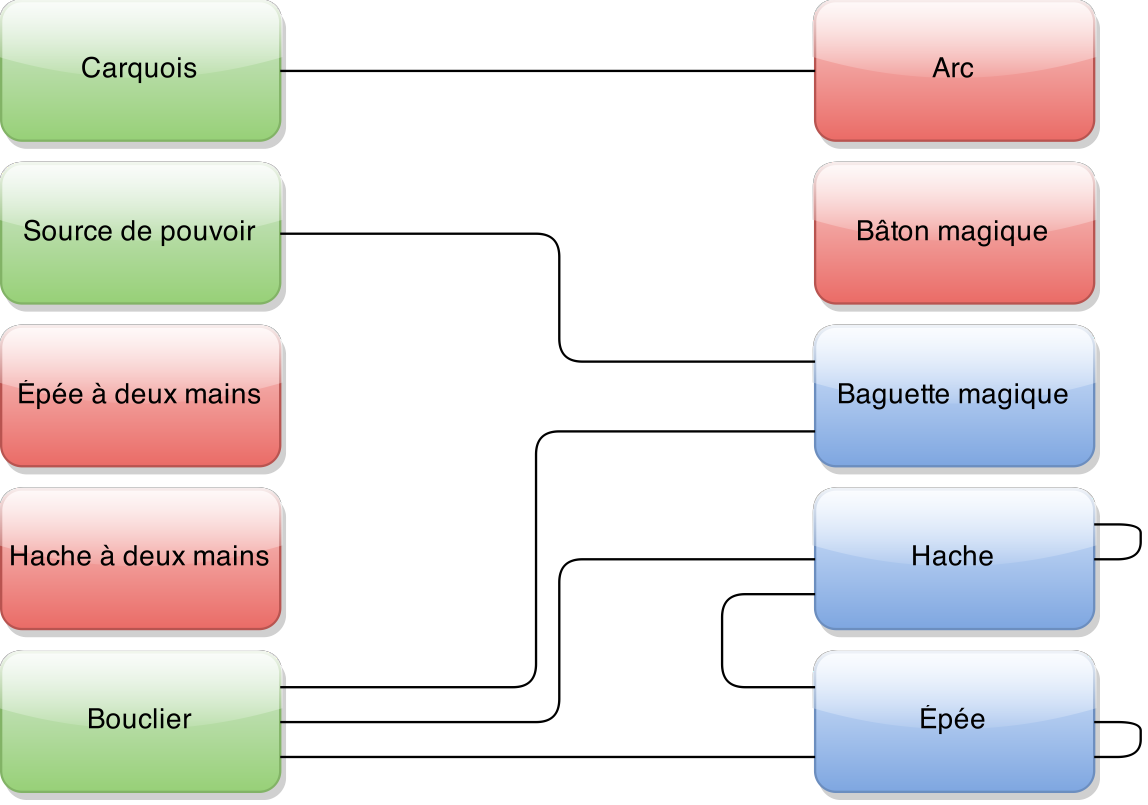
\includegraphics[width=0.8\textwidth]{EquipmentRestrictions}
	\caption{Restriction des armes}
	\label{fig:EquipmentRestrictions}
	\end{center}
\end{figure}
\subsubsection{Critères d'une arme}
Une arme est dotée de caractéristiques obligatoires qui apparaitront sur toutes les armes lootée dans le jeu:
\begin{multicols}{2}
\begin{itemize}
    \item Vitesse d'attaque initial
\end{itemize}
\end{multicols}
Elle est aussi dotée de caractéristiques optionnelles qui peuvent y figurées, certains de ces caractéristiques apparaissent obligatoirement selon le type d'objet:
\begin{multicols}{2}
\begin{itemize}
	\item Dégâts
    \item Dégâts magique
    \item Force
    \item Agilité
    \item Vitalité
    \item Magie
\end{itemize}
\end{multicols}
\subsubsection{Spécialités des type d'armes}
\begin{description}[labelindent=1cm]
    \item[Épée] Arme à une main avec la plus grande vitesse d'attaque
    \item[Épée à deux mains] Arme à deux mains avec la plus grande vitesse d'attaque
    \item[Hache] Arme à une main avec le plus de dégâts
    \item[Hache à deux mains] Arme à deux mains avec le plus de dégâts
    \item[Baguette magique] Permet d'avoir une source de pouvoir équipé en même temps.
    \item[Bâton magique] Possède de haut dégâts magiques
    \item[Arc] Haut dégâts physique à distance
\end{description}
\subsubsection{Épée}
L'épée apporte toujours ces caractéristiques :
\begin{table}[H]
\begin{center}
\begin{tabular}{| l | c | c | c |}
  \hline      
  Niveau 					& 1 & 2 & 3\\ \hline \hline                 
  Vitesse d'attaque initial	& 1.40 & 1.40 & 1.40\\ \hline
  Dégâts 					& 30 - 50 & 60 - 90 & 110 - 160\\ \hline
\end{tabular}
\caption{Valeurs des caractéristiques obligatoires de l'épée}
\end{center}
\end{table}
Elle apporte aussi 2 à 4 de ces caractéristiques :
\begin{table}[H]
\begin{center}
\begin{tabular}{| l | c | c | c |}
  \hline      
  Niveau 				& 1 & 2 & 3\\ \hline \hline                 
  Force 				& 3 - 10 & 15 - 30 & 45 - 100\\ \hline
  Agilité 				& 1 - 5 & 7 - 25 & 35 - 80\\ \hline
  Vitalité 				& 3 - 10 & 15 - 30 & 45 - 100\\ \hline
  Magie 				& 1 - 5 & 7 - 25 & 35 - 80\\ \hline
  Dégâts magiques 		& 5 - 10 & 20 - 40 & 50 - 80\\ \hline
\end{tabular}
\caption{Valeurs des caractéristiques optionnelles de l'épée}
\end{center}
\end{table}
\subsubsection{Épée à deux mains}
L'épée à deux mains apporte toujours ces caractéristiques :
\begin{table}[H]
\begin{center}
\begin{tabular}{| l | c | c | c |}
  \hline      
  Niveau 				& 1 & 2 & 3\\ \hline \hline                 
  Force 				& 3 - 10 & 15 - 30 & 45 - 100\\ \hline
  Vitesse d'attaque initial	& 1.10 & 1.10 & 1.10\\ \hline
  Dégâts 				& 65 - 110 & 120 - 190 & 230 - 360\\ \hline
\end{tabular}
\caption{Valeurs des caractéristiques obligatoires de l'épée à deux mains}
\end{center}
\end{table}
Elle apporte aussi 1 à 3 de ces caractéristiques :
\begin{table}[H]
\begin{center}
\begin{tabular}{| l | c | c | c |}
  \hline      
  Niveau 				& 1 & 2 & 3\\ \hline \hline
  Vitalité 				& 3 - 10 & 15 - 30 & 45 - 100\\ \hline
  Magie 				& 1 - 5 & 7 - 25 & 35 - 80\\ \hline
  Dégâts magiques 		& 3 - 15 & 25 - 45 & 60 - 90\\ \hline
  Régénération de vie 	& 5 - 50  & 80 - 275 & 375 - 750\\ \hline
  Régénération de mana 	& 1 - 3  & 4 - 10 & 11 - 15\\ \hline
\end{tabular}
\caption{Valeurs des caractéristiques optionnelles de l'épée à deux mains}
\end{center}
\end{table}
\subsubsection{Hache}
La hache apporte toujours ces caractéristiques :
\begin{table}[H]
\begin{center}
\begin{tabular}{| l | c | c | c |}
  \hline      
  Niveau 				& 1 & 2 & 3\\ \hline \hline                 
  Force 				& 3 - 10 & 15 - 30 & 45 - 100\\ \hline
  Vitesse d'attaque initial	& 1.30 & 1.30 & 1.30\\ \hline
  Dégâts 				& 30 - 50 & 60 - 90 & 110 - 160\\ \hline
\end{tabular}
\caption{Valeurs des caractéristiques obligatoires de la hache}
\end{center}
\end{table}
Elle apporte aussi 1 à 3 de ces caractéristiques :
\begin{table}[H]
\begin{center}
\begin{tabular}{| l | c | c | c |}
  \hline      
  Niveau 				& 1 & 2 & 3\\ \hline \hline
  Magie 				& 1 - 5 & 7 - 25 & 35 - 80\\ \hline
  Vitalité 				& 3 - 10 & 15 - 30 & 45 - 100\\ \hline
  Dégâts magiques 		& 3 - 10 & 20 - 40 & 50 - 80\\ \hline
\end{tabular}
\caption{Valeurs des caractéristiques optionnelles de la hache}
\end{center}
\end{table}
\subsubsection{Hache à deux mains}
La hache à deux mains apporte toujours ces caractéristiques :
\begin{table}[H]
\begin{center}
\begin{tabular}{| l | c | c | c |}
  \hline      
  Niveau 				& 1 & 2 & 3\\ \hline \hline                 
  Force 				& 3 - 10 & 15 - 30 & 45 - 100\\ \hline
  Vitalité 				& 3 - 10 & 15 - 30 & 45 - 100\\ \hline
  Vitesse d'attaque initial	& 1.00 & 1.00 & 1.00\\ \hline
  Dégâts 				& 65 - 110 & 120 - 190 & 230 - 360\\ \hline
\end{tabular}
\caption{Valeurs des caractéristiques obligatoires de la hache à deux mains}
\end{center}
\end{table}
Elle apporte aussi 0 à 2 de ces caractéristiques :
\begin{table}[H]
\begin{center}
\begin{tabular}{| l | c | c | c |}
  \hline      
  Niveau 				& 1 & 2 & 3\\ \hline \hline
  Magie 				& 1 - 5 & 7 - 25 & 35 - 80\\ \hline
  Dégâts magiques 		& 3 - 15 & 25 - 45 & 60 - 90\\ \hline
  Régénération de vie 	& 5 - 50  & 80 - 275 & 375 - 750\\ \hline
  Régénération de mana 	& 1 - 3  & 4 - 10 & 11 - 15\\ \hline
\end{tabular}
\caption{Valeurs des caractéristiques optionnelles de la hache à deux mains}
\end{center}
\end{table}
\subsubsection{Baguette magique}
La baguette magique apporte toujours ces caractéristiques :
\begin{table}[H]
\begin{center}
\begin{tabular}{| l | c | c | c |}
  \hline      
  Niveau 				& 1 & 2 & 3\\ \hline \hline
  Magie 				& 3 - 10 & 15 - 30 & 45 - 100\\ \hline
  Vitesse d'attaque initial	& 1.40 & 1.40 & 1.40\\ \hline
  Dégâts magiques 		& 30 - 50 & 60 - 90 & 110 - 160\\ \hline
\end{tabular}
\caption{Valeurs des caractéristiques obligatoires de la baguette magique}
\end{center}
\end{table}
Elle apporte aussi 1 à 2 de ces caractéristiques :
\begin{table}[H]
\begin{center}
\begin{tabular}{| l | c | c | c |}
  \hline      
  Niveau 				& 1 & 2 & 3\\ \hline \hline
  Agilité 				& 3 - 10 & 15 - 30 & 45 - 100\\ \hline
  Vitalité 				& 3 - 10 & 15 - 30 & 45 - 100\\ \hline
\end{tabular}
\caption{Valeurs des caractéristiques optionnelles de la baguette magique}
\end{center}
\end{table}
\subsubsection{Bâton magique}
Le bâton magique apporte toujours ces caractéristiques :
\begin{table}[H]
\begin{center}
\begin{tabular}{| l | c | c | c |}
  \hline      
  Niveau 				& 1 & 2 & 3\\ \hline \hline
  Magie 				& 3 - 10 & 15 - 30 & 45 - 100\\ \hline
  Vitesse d'attaque initial	& 1.20 & 1.20 & 1.20\\ \hline
  Dégâts magiques 		& 65 - 110 & 120 - 190 & 230 - 360\\ \hline
\end{tabular}
\caption{Valeurs des caractéristiques obligatoires du bâton magique}
\end{center}
\end{table}
Il apporte aussi 1 à 2 de ces caractéristiques :
\begin{table}[H]
\begin{center}
\begin{tabular}{| l | c | c | c |}
  \hline      
  Niveau 				& 1 & 2 & 3\\ \hline \hline
  Agilité 				& 3 - 10 & 15 - 30 & 45 - 100\\ \hline
  Vitalité 				& 3 - 10 & 15 - 30 & 45 - 100\\ \hline
  Régénération de vie 	& 5 - 50  & 80 - 275 & 375 - 750\\ \hline
  Régénération de mana 	& 1 - 3  & 4 - 10 & 11 - 15\\ \hline
\end{tabular}
\caption{Valeurs des caractéristiques optionnelles du bâton magique}
\end{center}
\end{table}
\subsubsection{Arc}
L'arc apporte toujours ces caractéristiques :
\begin{table}[H]
\begin{center}
\begin{tabular}{| l | c | c | c |}
  \hline      
  Niveau 				& 1 & 2 & 3\\ \hline \hline
  Agilité 				& 3 - 10 & 15 - 30 & 45 - 100\\ \hline
  Vitesse d'attaque initial	& 1.30 & 1.30 & 1.30\\ \hline
  Dégâts 				& 30 - 50 & 60 - 90 & 110 - 160\\ \hline
\end{tabular}
\caption{Valeurs des caractéristiques obligatoires de l'arc}
\end{center}
\end{table}
Il apporte aussi 1 à 3 de ces caractéristiques :
\begin{table}[H]
\begin{center}
\begin{tabular}{| l | c | c | c |}
  \hline      
  Niveau 				& 1 & 2 & 3\\ \hline \hline                 
  Force 				& 3 - 10 & 15 - 30 & 45 - 100\\ \hline
  Vitalité 				& 3 - 10 & 15 - 30 & 45 - 100\\ \hline
  Magie 				& 1 - 5 & 7 - 25 & 35 - 80\\ \hline
  Dégâts magiques 		& 3 - 10 & 20 - 40 & 50 - 80\\ \hline
\end{tabular}
\caption{Valeurs des caractéristiques optionnelles de l'arc}
\end{center}
\end{table}
\subsection{Armures}
\begin{multicols}{2}
\begin{itemize}
    \item Tête
    \item Épaules
    \item Corps
    \item Mains
    \item Jambes
    \item Pieds
\end{itemize}
\end{multicols}
\subsubsection{Tête}
Une armure pour la tête apporte obligatoirement ces caractéristiques :
\begin{table}[H]
\begin{center}
\begin{tabular}{| l | c | c | c |}
  \hline      
  Niveau 				& 1 & 2 & 3\\ \hline \hline
  Vitalité 				& 3 - 10 & 15 - 30 & 45 - 100\\ \hline
  Armure 				& 3 - 10 & 15 - 30 & 45 - 100\\ \hline
\end{tabular}
\caption{Valeurs des caractéristiques obligatoire de l'armure pour la tête}
\end{center}
\end{table}
Elle apporte aussi 0 à 2 de ces caractéristiques :
\begin{table}[H]
\begin{center}
\begin{tabular}{| l | c | c | c |}
  \hline      
  Niveau 				& 1 & 2 & 3\\ \hline \hline                 
  Force 				& 3 - 10 & 15 - 30 & 45 - 100\\ \hline
  Agilité 				& 3 - 10 & 15 - 30 & 45 - 100\\ \hline
  Magie 				& 3 - 10 & 15 - 30 & 45 - 100\\ \hline
  Resistance magique 	& 3 - 10 & 15 - 30 & 45 - 100\\ \hline
  Régénération de vie 	& 5 - 50  & 80 - 275 & 375 - 750\\ \hline
  Régénération de mana 	& 1 - 3  & 4 - 10 & 11 - 15\\ \hline
\end{tabular}
\caption{Valeurs des caractéristiques optionnelles de l'armure pour la tête}
\end{center}
\end{table}
\subsubsection{Épaules}
Une armure pour les épaules apporte obligatoirement ces caractéristiques :
\begin{table}[H]
\begin{center}
\begin{tabular}{| l | c | c | c |}
  \hline      
  Niveau 				& 1 & 2 & 3\\ \hline \hline
  Armure 				& 3 - 10 & 15 - 30 & 45 - 100\\ \hline
\end{tabular}
\caption{Valeurs des caractéristiques obligatoire de l'armure pour les épaules}
\end{center}
\end{table}
Elle apporte aussi 1 à 3 de ces caractéristiques :
\begin{table}[H]
\begin{center}
\begin{tabular}{| l | c | c | c |}
  \hline      
  Niveau 				& 1 & 2 & 3\\ \hline \hline                 
  Force 				& 3 - 10 & 15 - 30 & 45 - 100\\ \hline
  Agilité 				& 3 - 10 & 15 - 30 & 45 - 100\\ \hline
  Vitalité 				& 3 - 10 & 15 - 30 & 45 - 100\\ \hline
  Magie 				& 3 - 10 & 15 - 30 & 45 - 100\\ \hline
  Resistance magique 	& 3 - 10 & 15 - 30 & 45 - 100\\ \hline
\end{tabular}
\caption{Valeurs des caractéristiques optionnelles de l'armure pour les épaules}
\end{center}
\end{table}
\subsubsection{Corps}
Une armure pour le corps apporte obligatoirement ces caractéristiques :
\begin{table}[H]
\begin{center}
\begin{tabular}{| l | c | c | c |}
  \hline      
  Niveau 				& 1 & 2 & 3\\ \hline \hline
  Armure 				& 3 - 10 & 15 - 30 & 45 - 100\\ \hline
\end{tabular}
\caption{Valeurs des caractéristiques obligatoire de l'armure pour le corps}
\end{center}
\end{table}
Elle apporte aussi 1 à 3 de ces caractéristiques :
\begin{table}[H]
\begin{center}
\begin{tabular}{| l | c | c | c |}
  \hline      
  Niveau 				& 1 & 2 & 3\\ \hline \hline                 
  Force 				& 3 - 10 & 15 - 30 & 45 - 100\\ \hline
  Agilité 				& 3 - 10 & 15 - 30 & 45 - 100\\ \hline
  Vitalité 				& 3 - 10 & 15 - 30 & 45 - 100\\ \hline
  Magie 				& 3 - 10 & 15 - 30 & 45 - 100\\ \hline
  Resistance magique 	& 3 - 10 & 15 - 30 & 45 - 100\\ \hline
  Régénération de vie 	& 5 - 50  & 80 - 275 & 375 - 750\\ \hline
  Régénération de mana 	& 1 - 3  & 4 - 10 & 11 - 15\\ \hline
\end{tabular}
\caption{Valeurs des caractéristiques optionnelles de l'armure pour le corps}
\end{center}
\end{table}
\subsubsection{Mains}
Une armure pour les mains apporte obligatoirement ces caractéristiques :
\begin{table}[H]
\begin{center}
\begin{tabular}{| l | c | c | c |}
  \hline      
  Niveau 				& 1 & 2 & 3\\ \hline \hline
  Agilité 				& 3 - 10 & 15 - 30 & 45 - 100\\ \hline
  Armure 				& 3 - 10 & 15 - 30 & 45 - 100\\ \hline
\end{tabular}
\caption{Valeurs des caractéristiques obligatoire de l'armure pour les mains}
\end{center}
\end{table}
Elle apporte aussi 0 à 2 de ces caractéristiques :
\begin{table}[H]
\begin{center}
\begin{tabular}{| l | c | c | c |}
  \hline      
  Niveau 				& 1 & 2 & 3\\ \hline \hline                 
  Force 				& 3 - 10 & 15 - 30 & 45 - 100\\ \hline
  Vitalité 				& 3 - 10 & 15 - 30 & 45 - 100\\ \hline
  Magie 				& 3 - 10 & 15 - 30 & 45 - 100\\ \hline
  Resistance magique 	& 3 - 10 & 15 - 30 & 45 - 100\\ \hline
\end{tabular}
\caption{Valeurs des caractéristiques optionnelles de l'armure pour les mains}
\end{center}
\end{table}
\subsubsection{Jambes}
Une armure pour les jambes apporte obligatoirement ces caractéristiques :
\begin{table}[H]
\begin{center}
\begin{tabular}{| l | c | c | c |}
  \hline      
  Niveau 				& 1 & 2 & 3\\ \hline \hline
  Armure 				& 3 - 10 & 15 - 30 & 45 - 100\\ \hline
\end{tabular}
\caption{Valeurs des caractéristiques obligatoire de l'armure pour les jambes}
\end{center}
\end{table}
Elle apporte aussi 1 à 3 de ces caractéristiques :
\begin{table}[H]
\begin{center}
\begin{tabular}{| l | c | c | c |}
  \hline      
  Niveau 				& 1 & 2 & 3\\ \hline \hline                 
  Force 				& 3 - 10 & 15 - 30 & 45 - 100\\ \hline
  Agilité 				& 3 - 10 & 15 - 30 & 45 - 100\\ \hline
  Vitalité 				& 3 - 10 & 15 - 30 & 45 - 100\\ \hline
  Magie 				& 3 - 10 & 15 - 30 & 45 - 100\\ \hline
  Resistance magique 	& 3 - 10 & 15 - 30 & 45 - 100\\ \hline
\end{tabular}
\caption{Valeurs des caractéristiques optionnelles de l'armure pour les jambes}
\end{center}
\end{table}
\subsubsection{Pieds}
Une armure pour les pieds apporte obligatoirement ces caractéristiques :
\begin{table}[H]
\begin{center}
\begin{tabular}{| l | c | c | c |}
  \hline      
  Niveau 				& 1 & 2 & 3\\ \hline \hline
  Agilité 				& 3 - 10 & 15 - 30 & 45 - 100\\ \hline
  Armure 				& 3 - 10 & 15 - 30 & 45 - 100\\ \hline
\end{tabular}
\caption{Valeurs des caractéristiques obligatoire de l'armure pour les pieds}
\end{center}
\end{table}
Elle apporte aussi 0 à 2 de ces caractéristiques :
\begin{table}[H]
\begin{center}
\begin{tabular}{| l | c | c | c |}
  \hline      
  Niveau 				& 1 & 2 & 3\\ \hline \hline                 
  Force 				& 3 - 10 & 15 - 30 & 45 - 100\\ \hline
  Vitalité 				& 3 - 10 & 15 - 30 & 45 - 100\\ \hline
  Magie 				& 3 - 10 & 15 - 30 & 45 - 100\\ \hline
  Resistance magique 	& 3 - 10 & 15 - 30 & 45 - 100\\ \hline
\end{tabular}
\caption{Valeurs des caractéristiques optionnelles de l'armure pour les pieds}
\end{center}
\end{table}
\section{Sorts}
\subsection{Sort -- Bleed}
\emph{Bleed} ou saigné en français, est un sort qui inflige des dégâts continue à un ou plusieurs ennemis. Il inflige \textbf{200\%} de dégâts par secondes pendant \textbf{5} secondes dans un rayon de \textbf{10} mètres.

Le sort coûte \textbf{50} mana.\\

Disponible pour les armes suivants :
\begin{multicols}{2}
\begin{itemize}
    \item Épée à une main
    \item Hache à une main
    \item Épée à deux mains
    \item Hache à deux mains
\end{itemize}
\end{multicols}
\subsection{Sort -- Cripple}
\emph{Cripple} ou estropier en français, est un sort qui ralenti la vitesse de déplacement de l'ennemi de \textbf{80\%} et aussi sa vitesse d'attaque de \textbf{80\%} pendant \textbf{5} secondes. Le sort inflige aussi \textbf{140\%} de dégâts.

Le sort coûte \textbf{50} mana.\\

Disponible pour les armes suivants :
\begin{multicols}{2}
\begin{itemize}
    \item Épée à une main
    \item Hache à une main
\end{itemize}
\end{multicols}
\subsection{Sort -- Rapid Attack}
\emph{Rapid Attack} ou attaque rapide en français, est un sort qui augmente la vitesse d'attaque du personnage de \textbf{50\%} pendant \textbf{5} secondes.

Le sort coûte \textbf{50} mana.\\

Disponible pour les armes suivants :
\begin{multicols}{2}
\begin{itemize}
    \item Épée à une main
    \item Hache à une main
    \item Arc
\end{itemize}
\end{multicols}
\subsection{Sort -- Smash}
\emph{Smash} ou écraser en français, est un sort qui inflige \textbf{300\%} de dégâts dans un rayon de \textbf{10} mètres.

Le sort coûte \textbf{50} mana.\\

Disponible pour les armes suivants :
\begin{multicols}{2}
\begin{itemize}
    \item Épée à deux mains
    \item Hache à deux mains
\end{itemize}
\end{multicols}
\subsection{Sort -- Knock-out \& Freeze}
\emph{Knock-out} ou assommer en français, est un sort qui assomme les ennemis pendant \textbf{3} secondes et inflige \textbf{140\%} de dégâts dans un rayon de \textbf{6} mètres.

Le sort coûte \textbf{50} mana.\\

Disponible pour les armes suivants :
\begin{multicols}{2}
\begin{itemize}
    \item Épée à deux mains
    \item Hache à deux mains
\end{itemize}
\end{multicols}
\subsection{Sort -- Freeze}
\emph{Freeze} ou geler en français, est un sort qui gèle les ennemis pendant \textbf{3} secondes et inflige \textbf{140\%} de dégâts magiques dans un rayon de \textbf{6} mètres.

Le sort coûte \textbf{50} mana.\\

Disponible pour les armes suivants :
\begin{multicols}{2}
\begin{itemize}
    \item Bâton magique
    \item Baguette magique
\end{itemize}
\end{multicols}
\subsection{Sort -- Armor-up}
\emph{Armor-up} ou augmenter l'armure en français, est un sort qui augmente l'armure et la résistance magique du personnage de \textbf{100\%} pendant \textbf{5} secondes.

Le sort coûte \textbf{50} mana.\\

Disponible pour les armes suivants :
\begin{multicols}{2}
\begin{itemize}
    \item Bâton magique
    \item Baguette magique
\end{itemize}
\end{multicols}
\subsection{Sort -- Fast}
\emph{Fast} ou rapide en français, est un sort qui augmente la vitesse de déplacement du personnage de \textbf{100\%} pendant \textbf{5} secondes.

Le sort coûte \textbf{50} mana.\\

Disponible pour les armes suivants :
\begin{multicols}{2}
\begin{itemize}
    \item Épée à une main
    \item Hache à une main
    \item Arc
\end{itemize}
\end{multicols}
\subsection{Sort -- Zone-Damage}
\emph{Zone-Damage} ou dégâts de zone en français, est un sort qui inflige \textbf{600\%} de dégâts dans un rayon de \textbf{15} mètres.

Il inflige \textbf{600\%} de dégâts magique si le personnage est équipé d'un bâton magique ou d'une baguette magique.

Le sort coûte \textbf{50} mana.\\

Disponible pour les armes suivants :
\begin{multicols}{2}
\begin{itemize}
    \item Bâton magique
    \item Baguette magique
    \item Arc
\end{itemize}
\end{multicols}
\section{Ennemis}
Il y a 3 ennemis de bases de différentes tailles : petite, moyenne et grande.
\subsection{Boss final -- Hel}
\section{Monde}
Le monde du jeu est basé sur un concept simple. Le personnage commence dans un village (base principale) où il peut trouver un coffre et un portail pour se téléporter.
Le portail mène vers un niveau (le terrain de combat) généré d'où il ne peut plus revenir dans le village sans mourir. Ce niveau est composé de 3 zone de difficultés, chacun plus difficile que l'autre.
\subsection{Village}
\subsubsection{Coffre}
\subsubsection{Portail}
\subsection{Terrain de combat}
\section{Interface utilisateur}

\section{Contrôles}
\newpage
% --------------------------------------------------
\chapter{Analyse organique}
\section{Monogame}
\begin{figure}[H]
	\begin{center}
	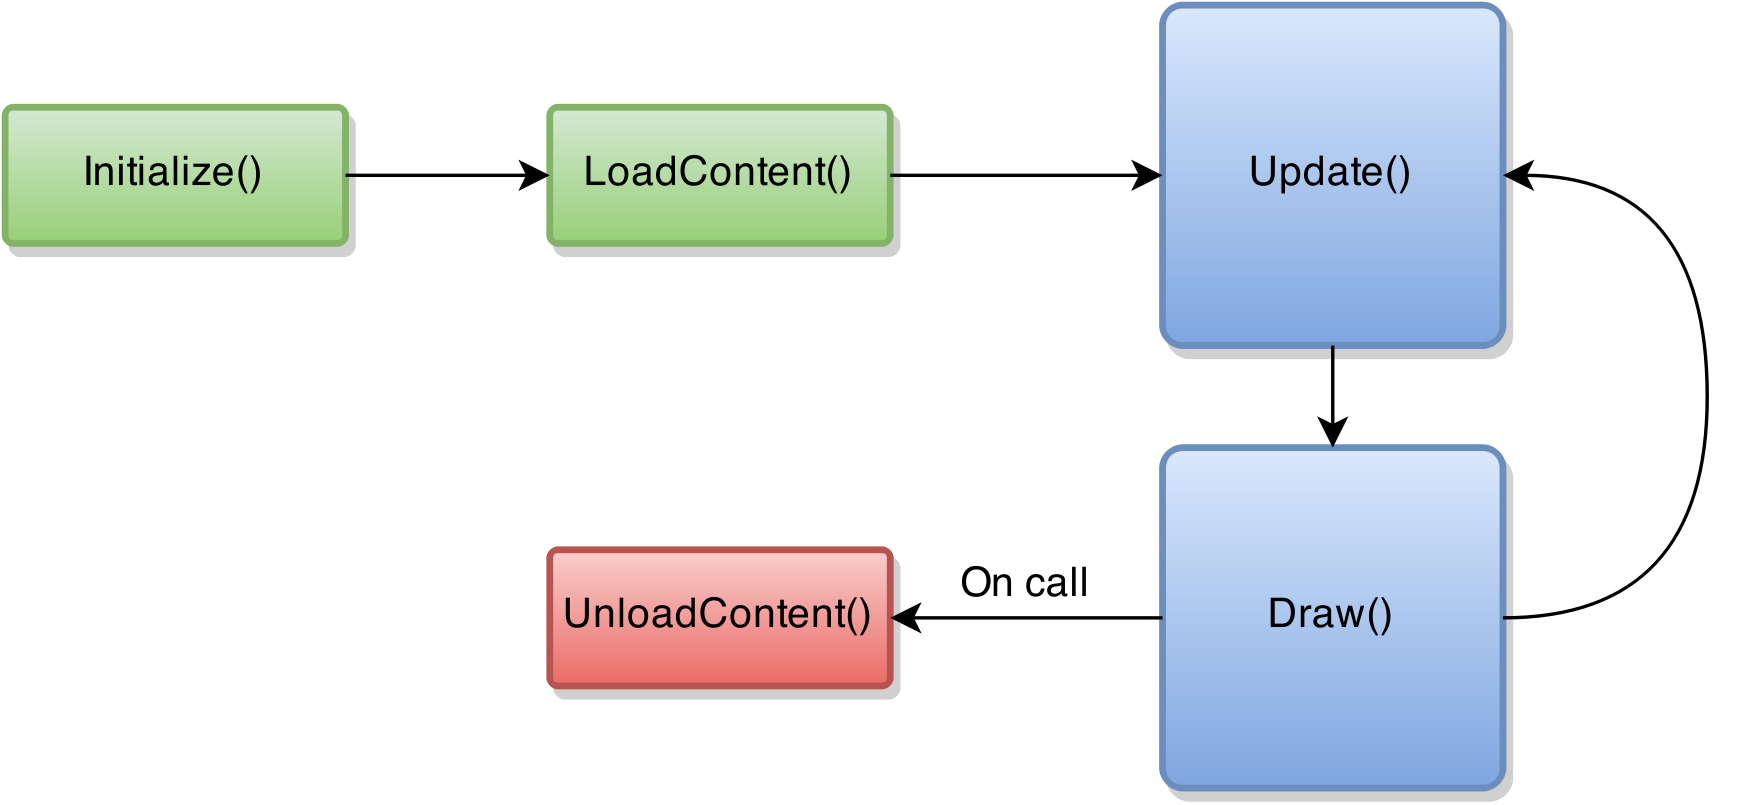
\includegraphics[width=0.8\textwidth]{loopmg}
	\caption{Boucle du framework MonoGame}
	\label{fig:loopmg}
	\end{center}
\end{figure}
\section{Génération de la carte}

\section{Gestion de l'écran}

\section{Gestion des entrées}

\newpage
% --------------------------------------------------
\chapter{Tests}

\newpage
% --------------------------------------------------
\chapter{Conclusion}

\newpage
% --------------------------------------------------
\chapter{Annexes}
\section{Planning}
Le planning du projet se décompose en plusieurs parties :\\
\begin{description}
	\item[Code backbone] Cœur du projet sur le quel le jeu se repose
	\item[Code essentiel] Éléments du jeu qui sont essentiels
	\item[Contenu] Contenu du jeu (Graphiques, Objets, etc.)
	\item[Tests] Tests pour vérifier l'intégralité du jeu
	\item[Poster] Poster préparer pour le projet
	\item[Documentation] Documentation technique du projet
\end{description}
\subsection{Initial}
% avril
\begin{figure}[H]
	\begin{center}
	\begin{ganttchart}[vgrid, hgrid, y unit title=1cm, y unit chart=0.7cm, x unit=0.8cm]{1}{14}
	    \gantttitle{Avril 2015}{14} \ganttnewline
	
	    \gantttitle{13}{1} % 1
	    \gantttitle{14}{1} % 2
	    \gantttitle{15}{1} % 3
	    \gantttitle{16}{1} % 4
	    \gantttitle{17}{1} % 5
	    \gantttitle{20}{1} % 6
	    \gantttitle{21}{1} % 7
	    \gantttitle{22}{1} % 8
	    \gantttitle{23}{1} % 9
	    \gantttitle{24}{1} % 10
	    \gantttitle{27}{1} % 11
	    \gantttitle{28}{1} % 12
	    \gantttitle{29}{1} % 13
	    \gantttitle{30}{1} \ganttnewline % 14
	    
	    \ganttbar[bar/.append style={fill=red}]{Code backbone}{6}{12} \ganttnewline
	    \ganttbar[bar/.append style={fill=red}]{Code essentiel}{12}{14} \ganttnewline
	    \ganttbar[bar/.append style={fill=blue}]{Poster}{13}{13} \ganttnewline
	    \ganttbar[bar/.append style={fill=blue}]{Documentation}{1}{14} \ganttnewline
	    \ganttmilestone{Rendu inter. doc. + poster}{14}
	\end{ganttchart}
	\caption{Planning initial du mois d'avril}
	\end{center}
\end{figure}
% mai 1
\begin{figure}[H]
	\begin{center}
	\begin{ganttchart}[vgrid, hgrid, y unit title=1cm, y unit chart=0.7cm, x unit=0.8cm]{1}{14}
	    \gantttitle{Mai 2015}{14} \ganttnewline
	
	    \gantttitle{4}{1} % 1
	    \gantttitle{5}{1} % 2
	    \gantttitle{6}{1} % 3
	    \gantttitle{7}{1} % 4
	    \gantttitle{8}{1} % 5
	    \gantttitle{11}{1} % 6
	    \gantttitle{12}{1} % 7
	    \gantttitle{13}{1} % 8
	    \gantttitle{15}{1} % 9
	    \gantttitle{18}{1} % 10
	    \gantttitle{19}{1} % 11
	    \gantttitle{20}{1} % 12
	    \gantttitle{21}{1} % 13
	    \gantttitle{22}{1} \ganttnewline % 14
	
	    \ganttbar[bar/.append style={fill=red}]{Code essentiel}{1}{8} \ganttnewline
	    \ganttbar[bar/.append style={fill=green}]{Contenu \& Équilibrage}{8}{14} \ganttnewline
	    \ganttbar[bar/.append style={fill=blue}]{Documentation}{1}{14}
	\end{ganttchart}
	\caption{Planning initial de la première partie du mois de mai}
	\end{center}
\end{figure}
% mai 2
\begin{figure}[H]
	\begin{center}
	\begin{ganttchart}[vgrid, hgrid, y unit title=1cm, y unit chart=0.7cm, x unit=0.8cm]{1}{6}
	    \gantttitle{Mai 2015}{4}
	    \gantttitle{Juin 2015}{2} \ganttnewline
	
	    \gantttitle{26}{1} % 1
	    \gantttitle{27}{1} % 2
	    \gantttitle{28}{1} % 3
	    \gantttitle{29}{1} % 4
	    \gantttitle{1}{2} \ganttnewline % 5
	
	    \ganttbar[bar/.append style={fill=green}]{Contenu \& Équilibrage}{1}{1} \ganttnewline
	    \ganttbar[bar/.append style={fill=yellow}]{Tests}{2}{4} \ganttnewline
	    \ganttbar[bar/.append style={fill=blue}]{Documentation}{1}{5} \ganttnewline
	    \ganttmilestone{Rendu final}{6}
	\end{ganttchart}
	\caption{Planning initial de la deuxième partie du mois de mai et le mois de juin}
	\end{center}
\end{figure}
\newpage
\subsection{Final}
\begin{figure}[H]
	\begin{center}
	\begin{ganttchart}[vgrid, hgrid, y unit title=1cm, y unit chart=0.7cm, x unit=0.8cm]{1}{14}
	    \gantttitle{Avril 2015}{14} \ganttnewline
	
	    \gantttitle{13}{1} % 1
	    \gantttitle{14}{1} % 2
	    \gantttitle{15}{1} % 3
	    \gantttitle{16}{1} % 4
	    \gantttitle{17}{1} % 5
	    \gantttitle{20}{1} % 6
	    \gantttitle{21}{1} % 7
	    \gantttitle{22}{1} % 8
	    \gantttitle{23}{1} % 9
	    \gantttitle{24}{1} % 10
	    \gantttitle{27}{1} % 11
	    \gantttitle{28}{1} % 12
	    \gantttitle{29}{1} % 13
	    \gantttitle{30}{1} \ganttnewline % 14
	    
	    \ganttbar[bar/.append style={fill=red}]{Code backbone}{7}{13} \ganttnewline
	    \ganttbar[bar/.append style={fill=red}]{Code essentiel}{0}{0} \ganttnewline
	    \ganttbar[bar/.append style={fill=blue}]{Poster}{11}{11}
	    \ganttbar[bar/.append style={fill=blue}]{}{13}{13}
	    \ganttnewline
	    \ganttbar[bar/.append style={fill=blue}]{Documentation}{1}{8}
	    \ganttbar[bar/.append style={fill=blue}]{}{11}{13}
	    \ganttnewline
	    \ganttmilestone{Rendu inter. doc. + poster}{14}
	\end{ganttchart}
	\caption{Planning final du mois d'avril}
	\end{center}
\end{figure}
% mai 1
\begin{figure}[H]
	\begin{center}
	\begin{ganttchart}[vgrid, hgrid, y unit title=1cm, y unit chart=0.7cm, x unit=0.8cm]{1}{14}
	    \gantttitle{Mai 2015}{14} \ganttnewline
	
	    \gantttitle{4}{1} % 1
	    \gantttitle{5}{1} % 2
	    \gantttitle{6}{1} % 3
	    \gantttitle{7}{1} % 4
	    \gantttitle{8}{1} % 5
	    \gantttitle{11}{1} % 6
	    \gantttitle{12}{1} % 7
	    \gantttitle{13}{1} % 8
	    \gantttitle{15}{1} % 9
	    \gantttitle{18}{1} % 10
	    \gantttitle{19}{1} % 11
	    \gantttitle{20}{1} % 12
	    \gantttitle{21}{1} % 13
	    \gantttitle{22}{1} \ganttnewline % 14
	
	    \ganttbar[bar/.append style={fill=red}]{Code essentiel}{0}{0} \ganttnewline
	    \ganttbar[bar/.append style={fill=green}]{Contenu \& Équilibrage}{0}{0} \ganttnewline
	    \ganttbar[bar/.append style={fill=blue}]{Documentation}{0}{0}
	\end{ganttchart}
	\caption{Planning final de la première partie du mois de mai}
	\end{center}
\end{figure}
% mai 2
\begin{figure}[H]
	\begin{center}
	\begin{ganttchart}[vgrid, hgrid, y unit title=1cm, y unit chart=0.7cm, x unit=0.8cm]{1}{6}
	    \gantttitle{Mai 2015}{4}
	    \gantttitle{Juin 2015}{2} \ganttnewline
	
	    \gantttitle{26}{1} % 1
	    \gantttitle{27}{1} % 2
	    \gantttitle{28}{1} % 3
	    \gantttitle{29}{1} % 4
	    \gantttitle{1}{2} \ganttnewline % 5
	
	    \ganttbar[bar/.append style={fill=green}]{Contenu \& Équilibrage}{0}{0} \ganttnewline
	    \ganttbar[bar/.append style={fill=yellow}]{Tests}{0}{0} \ganttnewline
	    \ganttbar[bar/.append style={fill=blue}]{Documentation}{0}{0} \ganttnewline
	    \ganttmilestone{Rendu final}{6}
	\end{ganttchart}
	\caption{Planning final de la deuxième partie du mois de mai et le mois de juin}
	\end{center}
\end{figure}
\newpage
% --------------------------------------------------
\listoffigures
\listoftables
\end{document}